\documentclass[a4paper, 12pt]{report}
\usepackage[utf8x]{inputenc}
\usepackage[italian]{babel}
%\usepackage[T1]{fontenc}
\usepackage{graphicx}
\usepackage{float}
\usepackage[centertags]{amsmath}
\usepackage{amsfonts}
\usepackage{amssymb}
\usepackage{amsthm}
\usepackage{newlfont}
\usepackage{fancyhdr}
\usepackage{tesisty}
\usepackage{algorithm2e}

%-------------------------------
% DEFINIZIONE DEGLI ENVIRONMENT
%-------------------------------

\newtheorem{obs}{Osservazione}[section]
\newenvironment{oss}
    {\begin{obs}\begin{normalfont}}
    {\hfill $\square \!\!\!\!\checkmark$ \end{normalfont}\end{obs}}

\newtheorem{pro}{Problema}[chapter]
\newenvironment{prob}
    {\begin{pro}\begin{normalfont}}
    {\hfill $\spadesuit$ \end{normalfont}\end{pro}}

\newtheorem{teor}{Teorema}[section]
\newenvironment{teorema}
    {\begin{teor}\textit }
    {\hfill  \end{teor}}

\newtheorem{defn}{Definizione}[section]
\newenvironment{de}
    {\begin{defn}\begin{normalfont}}
    {\hfill $\clubsuit$ \end{normalfont}\end{defn}}

\newtheorem{prop}{Proprietà}[section]
\newenvironment{pr}
{\begin{prop}\begin{normalfont}}
		{\hfill $\clubsuit$ \end{normalfont}\end{prop}}

%-----------------------------
% CONFIGURAZIONE DELLA PAGINA
%-----------------------------

\hfuzz2pt % Don't bother to report over-full boxes if over-edge is < 2pt

\fancypagestyle{plain}{
\fancyhead{}\renewcommand{\headrulewidth}{0pt} } \pagestyle{fancy}
\renewcommand{\chaptermark}[1]{\markboth{\small CAP. \thechapter \textit{ #1}} {} }
\renewcommand{\sectionmark}[1]{\markright{\small  \thesection \textit{ #1}} {} }
\voffset=-20pt    % distanza tra il limite superiore del foglio e l'intestazione
\headsep=40pt     % distanza  l'intestazione ed il testo del corpo
\hoffset=0 pt     % misura equivalente al margine sinistro
\textheight=620pt % altezza del corpo del testo
\textwidth=435pt  % larghezza del corpo del testo
\footskip=40pt    % distanza tra il testo del corpo ed il pie' di pagina
\fancyhead{}      % cancella qualsiasi impostazione per l'intestazione
\fancyfoot{}      % cancella qualsiasi impostazione per il pie' di pagina
\headwidth=435pt  % larghezza del'intestazione e del pie' di pagina
\fancyhead[R]{\rightmark} \fancyfoot[L]{\leftmark}
\fancyfoot[R]{\thepage}
\renewcommand{\headrulewidth}{0.3pt}   % spessore della linea dell'intestazione
\renewcommand{\footrulewidth}{0.3pt}   % spessore della linea del pi�di pagina

\numberwithin{equation}{section}
\renewcommand{\theequation}{\thesection.\arabic{equation}}




%--------------------------
% MODIFICARE DA QUI IN POI
%--------------------------

\begin{document}

\dedicate{Inserire la dedica}

\corso{DELL'AUTOMAZIONE} \titoloTesi{Realizzazione di un software per la stima del posizionamento di un corpo rigido con metodi di visione e validazione attraverso uso motore grafico} \anno{2016/2017}
\relatore{Daniele Carnevale}
 \autore{Luca Calacci}
\correlatore{Corrado Possieri\\ Domenico Cascone}

\baselineskip=25pt

\intestazione

%------------------------------------------------
% INTRODUZIONE E RINGRAZIAMENTI (NON MODIFICARE)
%------------------------------------------------

\fancypagestyle{plain}{
\fancyhead{}\renewcommand{\headrulewidth}{0pt} } \pagestyle{fancy}
\renewcommand{\chaptermark}[1]{\markboth{\small Cap. \thechapter \textit{ #1}} {} }
\renewcommand{\sectionmark}[1]{\markright{\small  \S \thesection \textit{ #1}} {} }
\voffset=-20pt                         % distanza tra il limite superiore del foglio e l'intestazione
\headsep=40pt                          % distanza  l'intestazione ed il testo del corpo
\hoffset=0pt                           % misura equivalente al margine sinistro
\textheight=620pt                      % altezza del corpo del testo
\textwidth=435pt                       % larghezza del corpo del testo
\footskip=40pt                         % distanza tra il testo del corpo ed il pie' di pagina
\fancyhead{}                           % cancella qualsiasi impostazione per l'intestazione
\fancyfoot{}                           % cancella qualsiasi impostazione per il pie' di pagina
\headwidth=435pt                       % larghezza del'intestazione e del pie' di pagina
\fancyhead[R]{\rightmark} \fancyfoot[L]{\leftmark}
\fancyfoot[R]{\thepage}
\renewcommand{\headrulewidth}{0.3pt}   % spessore della linea dell'intestazione
\renewcommand{\footrulewidth}{0.3pt}   % spessore della linea del pi�di pagina

\pagenumbering{Roman} \tableofcontents
\newpage

\pagenumbering{arabic}

\fancyhead[R]{Introduzione} \fancyfoot[L]{Introduzione}
\fancyfoot[R]{\thepage}

\chapter*{Ringraziamenti}
\addcontentsline{toc}{chapter}{Ringraziamenti}



\chapter*{Introduzione}
\addcontentsline{toc}{chapter}{Introduzione}

Questo lavoro di tesi nasce, inizialmente, da una richiesta di collaborazione da parte di Thales Alenia. In tale collaborazione si richiedeva lo studio, ed eventualmente la sintesi di una nuova soluzione ad un problema di stima. Quest'ultimo è stato così posto: \textbf{si considerino diverse misure della velocità angolare di un corpo rigido nello spazio, misure effettuate da due sensori differenti posti in posizioni e orientamenti diversi, si richiede, se possibile, di individuare la matrice di rotazione relativa tra il primo ed il secondo. Si deve essere in grado cioè di individuare l'orientamento del secondo sensore rispetto al primo.} Tale problema risulta particolarmente rilevante in ambito satellitare. Spesso infatti, in seguito alla messa in orbita di un satellite, quest'ultimo può subire deformazioni permanenti o transitorie. I sensori a bordo perciò possono risultare ruotati rispetto all'orientamento nominale e fornire una misura di velocità angolare scorretta. Se si individua però la trasformazione avvenuta, si è in grado di correggere la misura.

La prima metà di questo lavoro di tesi si concentrerà sulla soluzione del suddetto problema. Si preannuncia che la domanda posta ha risposta affermativa e si forniranno due soluzioni. In realtà tali soluzioni abbracceranno un problema più ampio, che comprende il primo, nel quale si richiede la stima di una trasformazione completa: matrice di rotazione e vettore di traslazione. Quest'ultimo, nel constesto su detto, potrebbe identificare un bias tra i due sensori. 
La prima soluzione si basa sull'utilizzo di tecniche di \textbf{Geometria algebrica} ed in particolare delle \textbf{basi di Groebner}. La seconda è un adattamento di un algoritmo spesso utilizzato in bio-informatica per il confronto di proteine, detto \textbf{Algoritmo di Kabsch} e garantirà una maggiore robustezza ai rumori in misura.

La seconda metà di questo lavoro invece nasce per curiosità personale ed abbraccia il settore della \textbf{visione artificiale}. Comprese le potenzialità degli strumenti individuati infatti, si è scelto di applicarli per fornire una soluzione ad un problema molto rilevante in contesti di \textbf{robotica mobile}. Si è pertanto progettato, implementato e testato un sistema di stima del posizionamento e orientamento assoluti di un osservatore mobile rispetto all'ambiente circostante, eventualemente ignoto, denominato \textbf{Visual Observer}. Tale strumento fa uso solo di fotocamere (almeno due) e può essere utilizzato in ambienti dove altri tipi di sensori falliscono o in concomitanza a soluzioni più comuni al fine di migliorare le prestazioni di stima. Ad esempio potrebbe essere utilizzato in ambienti al chiuso per calcolare la posizione di un drone.

Nel capitolo \ref{chap:mat} si introdurranno brevemente gli strumenti matematici utilizzati che si suppone possano essere non noti al lettore perché non trattati nel corso di studi.
Nel capitolo \ref{chap:visualObs} si motiverà e si esplicherà il funzionamento del sistema di posizionamento. Si renderà necessario, come vedremo, sia risolvere il problema di stima vero e proprio sia la generazione di un input valido per gli algoritmi individuati. Si preannuncia che sarà necessario: riuscire a misurare le coordinate dei punti del mondo utilizzando tecniche di \textbf{steroscopia}, scegliere un set di punti del mondo e "ricercare" gli stessi in un istante successivo al netto dello spostamento, mediante tecniche di \textbf{Feature Detection}, per procedere alla generazione di un set di coppie di "misure" da utilizzare come input agli algoritmi di stima individuati. Nel capitolo \ref{chap:stima} si risolverà pertanto il primo problema, invece nel \ref{chap:visione} si provvederà a fornire gli strumenti fini alla generazione del suddetto set.

Infine nel capitolo \ref{chap:implTest} si illustreranno le problematiche riscontrate, gli strumenti utilizzati e le soluzioni individuate durante l'implementazione del software. L'intera implementazione sarà improntata nel rispetto di un requisito di esecuzione realtime, si di poter rendere il sistema utilizzabile in contesti di controllo in feedback di robot mobili. Infine si testeranno le prestazioni e si validerà il sistema mediante l'uso di un motore grafico e l'interazione quindi con un ambiente virtuale.  

\fancyhf{} %elimina header/footer vecchi


\fancyhead[R]{\rightmark} \fancyhead[L]{\leftmark}
\fancyfoot[R]{\thepage}





%---------------------
% INCLUSIONE CAPITOLI
%---------------------


\chapter{Strumenti matematici}
\label{chap:mat}

\begin{minipage}{12cm}\textit{In questo capitolo verranno brevemente introdotti gli strumenti che verranno utilizzati in questo lavoro di tesi. Si introdurranno per prima gli strumenti di geometria algebrica quali: ideali, basi di Groebner, teoria dell'eliminazione. Successivamente si procederà ad illustrare la decomposizione SVD.}
\end{minipage}

\vspace*{1cm}

\section{Geometria algebrica}
\label{sec:Geom}

Per comprendere al meglio il lavoro svolto, conviene introdurre alcuni strumenti algebrici fondamentali. Si introdurranno le definizioni algebriche principali e successivamente si introdurrà il concetto di base di Groebner. 

\begin{defn}Si definisce \textbf{monomio} nelle variabili \textit{$x_1, ..., x_n$} un prodotto del tipo $x_1^{\alpha_1} \cdot ... \cdot x_n^{\alpha_n}$ dove gli $\alpha_i$ sono interi non negativi. Si utilizza inoltre la seguente notazione in forma vettoriale \textbf{$x^\alpha$}, dove $x = [x_1 \dots x_n]^T$ e $\alpha = [\alpha_1 \dots \alpha_n]^T$ 	
\end{defn}

\begin{defn}Si definisce \textbf{polinomio} \textit{p} con i coefficienti del campo $\mathbb{K}$ una combinazione $\mathbb{K}$-lineare finita di monomi del tipo
	\begin{center}
		$p = \sum_{\alpha}^{} a_\alpha x^{\alpha}$, $a_\alpha \in \mathbb{K}$
	\end{center}
	si usa indicare con \textbf{termine} l'elemento $\alpha$-esimo della sommatoria.	
\end{defn}

\begin{defn}
	Si usa indicare con $\mathbb{K}[x]$ l'insieme di tutti i polinomi che è possibile generare con monomi nelle variabili $x = [x_1 \dots x_n]^T$ e i coefficienti in $\mathbb{K}$.
\end{defn}

\begin{defn}
	Dato un set di polinomi $p_1(x), ...m p_s(x) \in \mathbb{K}$ si definisce \textbf{varietà affine} il seguente set
	\begin{center}
		$V(p_1(x), ..., p_s(x)) := \{x \in \mathbb{K}^n  \; | \; p_i(x) = 0, i = 1, ..., s \}$
	\end{center} 
\end{defn}

Date due varietà affini $V_1(p_1, ..., p_s)$ e $V_2(q_1, ..., q_t)$ è possibile definire le operazioni di unione e intersezione:
\begin{align}
	\nonumber
	& V_1 \cup V_2 = V(p_1q_1, ...,p_1q_t, p_2q_1, ..., p_2q_t, ..., p_sq_1, ..., p_sq_t), \\
	\nonumber
	& V_1 \cap V_2 = V(p_1, ..., p_s, q_1, ..., q_t).
\end{align}
Si può ora introdurre lo strumento fondamentale utilizzato e alcune sue proprietà.
	
\begin{defn}
	Si definisce \textbf{ideale} \textit{I} un subset di $\mathbb{K}[x]$ che gode delle seguenti proprieta:
	\begin{enumerate}
		\item $0 \in I $,
		\item $f, g \in I \Rightarrow f + g \in I$,
		\item $f \in I, h \in \mathbb{K}[x] \Rightarrow fh \in I$
	\end{enumerate}
\end{defn}
Un modo naturale di definire un ideale è generarlo a partire da un numero finito di polinomi $p_1, ..., p_s$:
\begin{center}
	$\left\langle p_1, ..., p_s \right\rangle := \left\lbrace p \in \mathbb{K}[x] \; | \; p = \sum_{i = 1}^{s} h_ip_i, h_i \in \mathbb{K}[x] \right\rbrace $
\end{center}
Siano $p_1, ..., p_s \in \mathbb{K}[x]$, se si considera un ideale $I = \left\langle p_1, ..., p_s \right\rangle$ esso può essere interpretato nella seguente maniera. Si considerino le seguenti equazioni,
\begin{align}
\nonumber
& p_1 = 0 \\
\nonumber
& \vdots\\
\nonumber
& p_s = 0
\end{align}
se considero $h_1, ..., h_s \in \mathbb{K}[x]$ tali equazioni \textbf{avranno come conseguenza} che
\begin{center}
	$h_1p_1 + ... + h_sp_s = 0$.
\end{center}
Si evince che si può considerare un ideale come l'insieme di tutte le conseguenze generate dal sistema di equazioni omogeneo formato dai polinomi generatori dell'ideale.
\begin{prop}
	Considerati i polinomi $p_1, ..., p_s$ e $q_1, ..., q_r \in \mathbb{K}[x]$ si ha che
	\begin{center}
		$\left\langle p_1, ..., p_s \right\rangle = \left\langle q_1, ..., q_r \right\rangle \Leftrightarrow V(p_1, ..., p_s) = V(q_1, ..., q_r)$
	\end{center}
\end{prop}
Dalla suddetta proprietà si evince che una varietà affine non viene alterata da un cambio di base, cioè essa è definita dall'ideale stesso e non dai polinomi usati come generatori.
\begin{defn}
	Data una varietà affine $V$ si definisce come l'\textbf{ideale di \textit{V}} il set di tutti i polinomi in $\mathbb{K}[x]$ che si annullano su di essa. In formule:
	\begin{center}
		$\mathbf{I}(V) := \left\lbrace p \in \mathbb{K}[x] \; | \; p(x) = 0, \quad \forall x \in V \right\rbrace $
	\end{center}
\end{defn}
In generale vale la seguente proprietà:
\begin{prop}
	Siano $p_1, ..., p_s \in \mathbb{K}[x]$ allora vale che $\left\langle p_1, ..., p_s \right\rangle \subseteq \mathbf{I}(V(p_1, ..., p_s))$. In generale il converso non vale.
\end{prop}
Si può definire infine il concetto di varietà affine di un ideale.
\begin{defn}
	Sia $I$ un ideale in $\mathbb{K}[x]$ il set
	\begin{center}
		$V(I) := \left\lbrace x \in \mathbb{K}^n \; | |; p(x) = 0, \forall p \in I \right\rbrace$
	\end{center}
	si dice \textbf{varietà affine dell'ideale} \textit{I}.
\end{defn}
Vale la seguente proprietà che sarà particolarmente utile alla definizione e determinazione delle preannunciate basi di Groebner.
\begin{prop}
	Sia \textit{I} un ideale in $\mathbb{K}[x]$ e siano $p_1, ..., p_s$ polinomi, allora vale che $V(I) = V(p_1, ..., p_s)$ per ogni base $\left\lbrace p_1, ..., p_s \right\rbrace$ di $I$
\end{prop}

Si consideri un polinomio nella variabile scalare s, del tipo $p = s^n + a_{n-1}s^{n-1} + \cdots + a_1s + a_0$, se considero un ulteriore polinomio $g \in \mathbb{K}[s]$, di grado $k \geq n$ è possibile dimostrare che esso è esprimibile con una relazione del tipo $g = qp + r$, dove $q$ è detto polinomio quoziente e $r$ resto. Inoltre vale che $deg(r) \le deg(g)$. In letteratura esistono diversi algoritmi volti a trovare i polinomio $q$ e $r$, ad esempio l'algoritmo di divisone tra polinomi che estende il concetto di divisione tra scalari.

Un fatto importante da notare è che se si considera un ideale $I = \left\langle g \right\rangle$, dove $g \in \mathbb{K}[x]$, è possibile allora verificare in modo semplice se un polinomio $p \in \mathbb{K}[x]$ appartiene all'ideale $I$ verificando che il resto della divisione di $p$ da $g$ è nullo.

Tale concetto, esteso, porta alla definizione delle suddette basi di Groebner e quindi alla determinazione di una base di ordine ridotto, in senso che verrà presto definito, che definisce un determinato ideale $I$. Al fine di poter estendere tale concetto è necessario poter definire un ordinamento totale tra i polinomi. Nel caso ad una sola variabile, un ordinamento naturale è quello di considerare il grado dei polinomi (l'esponente maggiore con cui compare la variabile del polinomio). Si può estendere tale approccio ma occorre stabilire un ordinamento lessicografico tra i monomi di cui un polinomio si compone. Tale ordinamento può essere definito in diversi modi, nel nostro caso useremo il seguente.

\begin{defn}
	Si considerino due monomi $x^{\alpha}$ e $x^{\beta}$, dove $x = [x_1 \; ... \; x_n]^T$ e $\alpha, \beta \in \mathbb{Z}^n$, si dice che $x^{\alpha}$ e $x^{\beta}$ sono \textbf{in ordine lessicografico}, in simboli $x^{\alpha} \ge_{Lex} x^{\beta}$, con $x_1 \ge x_2 \ge \cdots \ge x_n$ se vale che
	il primo elemento non nullo del vettore $\alpha-\beta$ è maggiore di zero.	
\end{defn}
Si fa notare che il precedente ordinamento è fortemente influenzato dall'ordinamento che si da alle variabili $x_i$, infatti al variare di tale ordinamento (e corrispettiva variazione dell'ordinamento sui vettori $\alpha$ e $\beta$) si ottengono ordinamenti diversi.

\begin{defn}
	Dato un polinomio $p \in \mathbb{K}[x]$ se si definisce un ordine lessicografico e si riscrive tale polinomio in modo ordinato, $ p = a_1x^{\alpha_1} + a_2x^{\alpha_2} + \cdots $,  si definiscono il \textbf{leading monomial} $LM(p) := x^{\alpha_1}$, il \textbf{leading coefficient} $LC(p) := a_1$ e il \textbf{leading terms} $LT(p) := a_1x^{\alpha_1}$
\end{defn}
Si può estendere quindi il concetto di divisione tra polinomi, al fine di ottenere un algoritmo multi-variabile in grado di dividere un polinomio per un set di polinomi. In altre parole dato un set di polinomi $p_1, ..., p_s$ e un polinomio $p$ appartenenti a $\mathbb{K}[x]$ è possibile trovare $q_1, ... , q_s, r \in \mathbb{K}[x]$ tali che $p = q_1p_1 + q_1p_2 + \cdots + q_sp_s + r$ e vale che o $r = 0$ oppure $r = c_1x^{\beta_1} + c_2x^{\beta_2} + \cdots $ e nessun $c_ix^{\beta_i}$ è divisibile per nessun $LT(p_j)$ con $i = 1,2,..., j = 1, 2,..., s$.

\begin{obs}
	Si può quindi facilmente capire che dato un ideale $I = \left\langle p_1, ..., p_s \right\rangle, p_i \in \mathbb{K}[x]$ e un ulteriore polinomio $p \in \mathbb{K}[x]$, quest'ultimo diviso per il set suddetto, si otterrà un resto nullo se e solo $ p \in I$. In altre parole si è trovato uno strumento per verificare se un polinomio è conseguenza di un ideale.
\end{obs}

Si riporta in seguito un algoritmo, chiamato \textbf{Multivariate division algoritmh}, atto a tale scopo. \\

\begin{algorithm}[H]
	\SetAlgoLined
	\KwData{una tupla ordinata $p_1, ..., p_s$ di polinomi $\in \mathbb{K}[x]$ e un polinomio $p \in \mathbb{K}[x]$}
	\KwResult{$q_1, ..., q_s, r \in \mathbb{K}[x]$}
	set $q_1 := 0, ..., q_s := 0$\;
	set r := 0\;
	set f := p\;
	\While{f $\neq$ 0}{
		i = 1; divisionOccurred = false\;
		\While{$i \leq s$ AND divisionOccurred == False}{
			\eIf{LT($p_i$) divide LT(f)}{
				$q_i = q_i + \frac{LT(f)}{LT(p_i)}$\;
				$f = f - \frac{LT(f)}{LT(p_i)}p_i$\;
				divisionOccurred = True\;
			}{
				$i = i + 1$\;
			}
		}
		\If{divisionOccurred == False}{
			$r = r + LT(f) $\;
			$f = f - LT(f) $\;
		}
	}
	\caption{Multivariate division algoritmh}
\end{algorithm}

\begin{prob}
	\label{prob:mvda}
	Il risultato del precedente algoritmo è fortemente dipendente dall'ordinamento dato ai polinomi $p_i$. Si vogliono trovare, se esistono, strumenti tali da rendere il calcolo del resto di tale divisione indipendente dall'ordinamento dato al set dei polinomi $p_i$.
\end{prob}

Il problema \ref{prob:mvda} costituisce la motivazione per introdurre le preannunciate basi di Groebner (ridotte), le quali, come si vedrà, permettono di risolvere tale problema.

\begin{defn}
	Si consideri l'ideale $I \subset \mathbb{K}[x]$ non vuoto, si fissi un ordinamento per i monomi e si definisca l'insieme
	\begin{center}
		$LT(I) := \left\lbrace cx^{\alpha} monomio \; | \; \exists f \in I \; \; \; t.c. \; \;  LT(f) = cx^{\alpha} \right\rbrace $
	\end{center} 
	e l'ideale dei leading terms generato da tale insieme $\left\langle LT(I) \right\rangle $.
	Un subset finito $G := \left\langle g_1, ..., g_m\right\rangle \subset I$ si dice una \textbf{base di Groebner} per l'ideale $I$ se vale
	\begin{center}
		$\left\langle LT(g_1), ..., LT(g_m) \right\rangle = \left\langle LT(I) \right\rangle$
	\end{center}
\end{defn}

\begin{prop}
	Sia $\left\langle \O \right\rangle := \{0\}$ il subset vuoto e sia esso per convenzione una base di Groebner per l'ideale vuoto, allora per ogni ideale esiste (non necessariamente unica) una base di Groebner che è una base per tale ideale.
\end{prop}

\begin{defn}
	Un polinomio $r \in \mathbb{K}[x]$ si dice \textbf{ridotto} rispetto ad un set $\left\lbrace g_1, ..., g_m \right\rbrace$, $g_i \in \mathbb{K}[x]$, se esso è esprimibile come una combinazione $\mathbb{K}$-lineare di termini nessuno dei quali è divisibile per nessuno dei $LT(g_1), ..., LT(g_m)$.
\end{defn}

\begin{defn}
	Una base di Groebner $\left\lbrace g_1, ..., g_m \right\rbrace$ si dice \textbf{ridotta} se vale che:
	\begin{enumerate}
		\item $LC(g_i) = 1, i = 1, ..., m$,
		\item $g_i$ è ridotto rispetto al set $\left\lbrace g_1, ...g_{i-1},g_{i+1}, ..., g_m \right\rbrace, i = 1, ..., m$
	\end{enumerate}
\end{defn}

\begin{prop}
	Per ogni ideale $I \subset \mathbb{K}[x]$ esiste un unica base di Groebner ridotta.
\end{prop}

\begin{prop}
	Sia $p \in \mathbb{K}[x]$ e $G$ una base di Groebner per l'ideale $I \subset \mathbb{K}[x]$. Allora il resto della divisione di $p$ per il set $G$ è unico indipendentemente dall'ordine dei polinomi $g_i$.
\end{prop}
Risulta abbastanza chiaro che l'uso delle basi di Groebner per definire un ideale permette di risolvere il problema \ref{prob:mvda}; infatti un polinomio $p \in I$ se e solo se vale che il resto della divisione tra $p$ e la base di Groebner di $I$ è nullo.
Si pone a questo punto il problema della determinazione di una base di Groebner dato un ideale I. A tal fine si può utilizzare l'algoritmo di Buchberger.

\begin{algorithm}[H]
	\SetAlgoLined
	\KwData{un set $p_1, ..., p_s$ di polinomi $\in \mathbb{K}[x]$}
	\KwResult{una base di Groebner $G$ per $\left\langle p_1, ..., p_s \right\rangle $}
	$G = \left\lbrace p_1, ..., p_s \right\rbrace $\;
	\Repeat{$G == $\^{G}}{
		\^{G} = G\;
		\ForEach{$p, q \in$ \^{G}, $p \neq q$}{
			$x^{\alpha} = LM(p)$; $x^{\beta} = LM(q)$\;
			$\gamma = (\gamma_1, ..., \gamma_n)$; $\gamma_i = max(\alpha_i, \beta_i)$\;
			$s = \frac{x^{\gamma}}{LT(p)}p - \frac{x^{\gamma}}{LT(q)}q$\;
			r := resto della divisione tra $s$ e il set \^{G}\;
			\If{$r \neq 0$}{
				$G = G \cup {r}$\;
			}
		}
	}
	
	\caption{Buchberger's algoritmh}
\end{algorithm}

\medskip
Si noti che il suddetto algoritmo non fornisce in genere una base di Groebner ridotta, infatti mantiene in G i polinomi $p_i$. 
Si fa notare che lo scopo del polinomio $s$ è quello di permettere cancellazioni tra i leading terms dei polinomi $p$ e $q$, ci si riferisce ad esso come il polinomio-S, in simboli $S(p,q)$. Infine la condizione di terminazione è corretta perché è possibile dimostrare che un set di polinomi $G = \{g_1, ..., g_m\}$ è una base di Groebner per un certo ideale $I$ se e solo se per ogni $i,j = 1,..., m , \; i\neq j$ il resto della divisione di $S(g_i, g_j)$ per il set $G$ è nullo (Buchberger's criterion). Si fa presto a capire che siccome per ogni coppia (p,q) si deve effettuare una divisione con tutti i polinomi in \^{G} ed inoltre per ogni iterazione si aggiungerà un polinomio a tale set, l'algoritmo risulta pesante dal punto di vista computazionale. Infatti, si può dimostrare che l'algoritmo è EXPSPACE-complesso, cioè con tempo di calcolo e occupazione di memoria esponenziali. In genere però esso risulta applicabile sui computer moderni.
Nel seguito della trattazione si utilizzerà il software Macaulay2 per il calcolo delle basi di Groebner di un dato ideale, il quale implementa proprio il suddetto algoritmo.


% --------- elimination theory
\subsubsection{Teoria dell'eliminazione}
Durante gli studi algebrici sicuramente ci si può essere imbattuti in un noto algoritmo detto: \textbf{Eliminazione di Gauss}. Quest'ultimo permette, dato un sistema lineare di equazioni - rappresentabile attraverso una matrice, attraverso operazioni elementari su sopraddetta matrice (operazioni che non ne alterano il rango), di ottenere una rappresentazione, in ipotesi di rango riga pieno, detta (quasi-)triangolare superiore. In tal modo si ottiene un sistema di equazioni in cui le ultime equazioni non dipendono da un certo numero delle prime variabili. Selezionando un certo numero delle ultime equazioni, è possibile ottenere un sotto-sistema in cui le prime variabili non compaiono (sono state eliminate). 
Tale approccio viene utilizzato per risolvere in maniera più semplice un sistema di equazioni, in ipotesi che possa essere fatto.

Tale concetto può essere esteso al caso polinomiale, non lineare, multi-variabile.

\begin{defn}
	Un set di polinomi $p_1, ..., p_m$, $p_i \in \mathbb{K}[x]$, si dice linearmente dipendente se esistono $c_1, ... c_m$ costanti non tutte nulle tale che $c_1p_1 + c_2p_2 + \, ... \, + c_mp_m = 0$. Altrimenti si dice \textbf{linearmente indipendente}.
	
	Un set di polinomi $p_1, ..., p_m$, $p_i \in \mathbb{K}[x]$, si dice algebricamente dipendente se esiste $q \in \mathbb{K}[y_1, \, ... \, , y_m]$ polinomio non nullo, tale che  $q(p_1, \, ..\, p_m) = 0 \in \mathbb{K}[x]$ (è il polinomio nullo). Altrimenti si dice \textbf{algebricamente indipendente}.
\end{defn}

Dato un ordinamento lessicografico $x_1 \ge_{Lex} x_2 \ge_{Lex} ... \ge_{Lex} x_n$ può essere possibile eliminare le prime $n-1$ variabili. Si dice infatti che tale ordine \textbf{elimina} $x_1, \, ... \, , x_{n-1}$.

\begin{defn}
	Dato un ordinamento lessicografico $x_1 \ge_{Lex} x_2 \ge_{Lex} ... \ge_{Lex} x_n$ e un ideale $I \subset \mathbb{K}[x]$ allora l'ideale
	\begin{center}
		$I_l = I \cap \mathbb{K}[x_{l+1}, \, ... \, x_{n}]$
	\end{center}
	si dice l'ideale di eliminazione di ordine $l$.
\end{defn} 
L'ideale di eliminazione di ordine $l$ può essere visto come l'insieme di tutte le conseguenze di un ideale nelle quali le prime $l$ variabili non compaiono.

Si può introdurre infine il teorema generale di eliminazione.
\begin{teor}
	\label{teo:elimination}
	Sia dato un ideale $I \subset \mathbb{K}[x_a, x_b]$ con $x_a \in \mathbb{R}^n_a, x_b \in \mathbb{R}^n_b$, $ n_a, n_b > 0$, $n = n_a + n_b$, e un ordinamento lessicografico $x_a \ge_{Lex} x_b$. Inoltre sia $G$ una base di Groebner ridotta per l'ideale $I$, calcolata in accordo a tale ordinamento. Allora vale che una base di Groebner per l'ideale di eliminazione di ordine $n_a$ è 
	\begin{center}
		$G_{n_a} = G \cap \mathbb{K}[x_b]$.
	\end{center}
\end{teor}

Mediante l'utilizzo delle basi di Groebner e il precedente teorema è possibile quindi estendere il concetto di eliminazione, per applicarlo a sistemi di equazioni omogenei multi-variabile polinomiali non lineari. In modo di ottenere delle conseguenze, sistemi omogenei di dimensione ridotta dello stesso tipo, che non contengano alcune variabili. Tale strumento può essere utilizzato per ottenere soluzioni analitiche ai problemi studiati. 

\section{Decomposizione ai valori singolari}
\label{sec:SVD}

In algebra lineare, la decomposizione ai valori singolari, detta anche SVD (dall'acronimo inglese Singular Value Decomposition), è una particolare fattorizzazione di una matrice basata sull'uso di autovalori e autovettori. 

\begin{defn}
	Data una matrice $M \in \mathbb{C}^{m \times n}$, si definisce decomposizione ai valori singolari o SVD la seguente decomposizione:
	\begin{center}
		$M = U \Sigma V^*$
	\end{center}
	dove $U$ è una matrice unitaria di dimensioni  $m\times m$, $\Sigma$ è una matrice diagonale rettangolare di dimensioni $m\times n$ e $V^*$ è la trasposta coniugata di una matrice unitaria $V$ di dimensioni $n\times n$.
	Si definiscono inoltre:
	\begin{enumerate}
		\item gli elementi di $\Sigma$ valori singolari della matrice $M$,
		\item le colonne di $U$ vettori singolari sinistri della matrice $M$,
		\item le righe di $V^*$ covettori singolari destri  della matrice $M$.		
	\end{enumerate}
\end{defn}

\begin{prop}
	Data una decomposizione SVD valgono le seguenti proprietà:
	\begin{enumerate}
		\item se $ m \le n$, allora $\Sigma = [\Sigma_0 \, \, 0]$, dove $\Sigma_0 = diag \{\sigma_1, ..., \sigma_m \}, \sigma_i \in \mathbb{R}, \sigma_i \ge 0$,
		\item se $ m > n$, allora $\Sigma = [\Sigma_0^T \, \, 0^T]^T$, dove $\Sigma_0 = diag \{\sigma_1, ..., \sigma_n \}, \sigma_i \in \mathbb{R}, \sigma_i \ge 0$,	 
		\item i valori singolari $\sigma_i$ non nulli di $M$ sono le radici quadrate degli autovalori della matrice $MM^*$ e $M^*M$,
		\item i vettori singolari di sinistra di $M$ sono gli autovettori di $MM^{*}$,
		\item i covettori singolari di destra di $M$ sono gli autovettori di $M^{*}M$ trasposti.
	\end{enumerate}
\end{prop}

Per il calcolo della decomposizione SVD sebbene è possibile procedere usando la definizione data, questo è sconsigliato perché inefficiente. Negli ultimi anni sono stati sviluppati diversi algoritmi atti allo scopo. Nello specifico si cita l'algoritmo Golub/Kahan utilizzato nelle recenti librerie matematiche come LAPACK, BLAS e CUBLAS.

In particolare si fa notare che questi algoritmi sono particolarmente efficienti quando la matrice da decomporre è quadrata.

La fattorizzazione SVD ha numerose applicazioni pratiche, infatti:
\begin{enumerate}
	\item il rango di una matrice è pari al numero di valori singolari maggiori di zero nella sua decomposizione SVD.
	\item può essere usata per il calcolo della matrice pseudo-inversa destra (o sinistra). Infatti sia $M \in \mathbb{C}^{m \times n}, rank(M) = m$ allora la sua decomposizione sarà $M = U [ \Sigma_0 \,\, 0 ] V^*, \Sigma_0 > 0, UU^* = I, VV^* = I$, allora una pseudo inversa destra per $M$ può essere calcolata come:
	\begin{center}
		$M^{R} = V 
		\begin{bmatrix}
			\Sigma_0^{-1} \\
			Z
		\end{bmatrix} U^*$
	\end{center} 
	dove $Z$ è una qualsiasi matrice che può essere anche nulla e $\Sigma_0^{-1}$ è sempre diagonale e cui elementi saranno del tipo $1/\sigma_i$.
	\item come vedremo nel paragrafo \ref{sec:kabsch} è particolarmente utile per risolvere problemi ai minimi quadratici.
\end{enumerate}
\chapter{Visual Observer}
\label{chap:visualObs}

\begin{minipage}{12cm}\textit{In questo capitolo verranno illustrate le motivazioni e le dinamiche che hanno portato alla decisione dell'implementazione di uno stimatore di posizione basato su visione. Inoltre verrà fornita una descrizione generica sulla logica di funzionamento; logica che verrà approfondita nei capitoli successivi.}
\end{minipage}

\vspace*{1cm}



\section{Motivazioni}
\label{sec:motivi}


\section{Approccio al problema}
\label{sec:approccio}



\chapter{Stima della matrice di trasformazione}
\label{chap:stima}

\begin{minipage}{12cm}\textit{In questo capitolo verrà trattato il problema della stima della matrice di trasformazione tra due set di coppie di punti. Tale problema, può essere ricondotto ad uno molto antico, noto come problema di Procrustes. Si studieranno due diversi approcci alla soluzione.}
\end{minipage}

\vspace*{1cm}

Come già preannunciato, obbiettivo di questo capitolo è quello di riuscire ad individuare la matrice di trasformazione tra due set di punti. Tali set si suppongono avere la stessa "forma", cioè essere delle grandezze strettamente correlate: ad esempio possono essere campioni della stessa quantità misurati da differenti sensori; oppure essere le coordinate di punti dello spazio in istanti del tempo diversi. Nel seguito si definirà il problema e si studieranno due soluzioni differenti atte a trovare, in forma analitica, la trasformazione in esame.  

%qua descrivo il problema...
\section{Il problema: Superimposizione di Procrustes}
\label{sec:problStima}
Il problema in esame si configura come una versione semplificata di un antico problema detto \textbf{superimposizione di Procrustes}. Nell'antica mitologia greca Procrustes, o Damaste, era un brigante solito aggredire i viaggiatori per poi smembrarli in modo di riuscire disporre le membra su di un tavolo di ferro. 
Per fortuna, il problema matematico in esame risulta meno cruento e può essere riassunto nel modo seguente: \textit{dati due corpi (N-dimensionali), attraverso solo operazioni di rotazione, traslazione e ridimensionamento, si deve riuscire a far combaciare il primo sul secondo in modo ottimo. L'ottimo viene valutato attraverso una quantità detta distanza di Procrustes.} Si dice che il primo viene super-imposto sul secondo; ovviamente qualora i due corpi abbiano la stessa forma la distanza di Procrustes sarà nulla. 
Tale problema risulta molto studiato in ambiti bioinformatici per comparare strutture di proteine. 

Nel resto del capitolo verrà però imposto un vincolo: \textit{i corpi posti a confronto non sono stati scalati.} Tale vincolo, permette di non dover considerare operazioni di ridimensionamento. Infatti, come già preannunciato nel capitolo \ref{chap:visualObs}, l'ambiente circostante si supporrà statico e quindi in nessun modo esso potrà essere ridimensionato.
Inoltre, adotteremo una struttura specifica per i corpi in esame: essi si suppongono essere dei politopi, descritti quindi dai loro vertici. In sostanza questo ci permette di dover tener conto di soli insiemi di punti. 




\section{Il metodo di Groebner}
\label{sec:groeb}
In questo paragrafo si presenta una metodologia di risoluzione del problema in esame mediante l'utilizzo degli strumenti di geometria algebrica. Si procederà prima allo studio del caso planare per poi estendere il risultato al caso spaziale.

\subsection{Il caso planare}
\label{sec:groeb:plan}
In questo paragrafo viene trattato il problema della matrice di trasformazione tra due set i punti nel piano, utilizzando gli strumenti di geometria algebrica visti nel paragrafo \ref{sec:Geom}. In particolare si vuole far ricorso al teorema (\ref{teo:elimination}), teorema dell'eliminazione, al fine di ottenere una soluzione analitica al problema.

Il primo passo è quello di definire un set di polinomi che possa essere utilizzato per definire un ideale di partenza. Tale ideale, come si vedrà, sarà impiegato come base per individuare un set di conseguenze (equazioni omogenee polinomiali), dalle quali si ricaverà sia la matrice di rotazione che il vettore di traslazione.

Procedendo con ordine, siano $w_1, w_1^{'}, w_2, w_2^{'} \in \mathbb{K}[w]^2$ (vettori polinomiali, crf. paragrafo \ref{sec:Geom}),  $t \in \mathbb{K}[t]^2$ e $R \in \mathbb{K}[r]^{2 \times 2}$, si definisce l'ideale base attraverso il seguente set di polinomi:
\begin{align}
	\begin{bmatrix}p_1 \\ p_2 \end{bmatrix} &:= w_1 - Rw_1^{'} - t,\\
	\begin{bmatrix}p_3 \\ p_4 \end{bmatrix} &:= w_2 - Rw_2^{'} - t, \\
	p_5 &:= det(R) - 1,\\
	p_{6} &:= (w_{2x} - w_{1x})^2 + (w_{2y} - w_{1y})^2 - (w_{2x}^{'} - w_{1x}^{'})^2 - (w_{2y}^{'} - w_{1y}^{'})^2
\end{align}
dove: 
\begin{equation}
	R := \begin{bmatrix}
	\,r_{11}, \,\, r_{12} \\
	-r_{12}, \,\, r_{11}
	\end{bmatrix}, \, t := \begin{bmatrix}	\,t_x \\ t_y\end{bmatrix}, w_i := \begin{bmatrix}	\,w_{ix} \\ w_{iy}\end{bmatrix}
\end{equation}
Si nota che i primi due blocchi di polinomi rappresentano la relazione di trasformazione tra i punti, il terzo e la forma scelta per $R$ la definiscono come ortonormale e con determinante (nel campo polinomiale) pari ad 1, cioè $R$ è una matrice di rotazione. Per quanto riguarda l'ultimo polinomio, esso identifica la relazione di rigidità tra i punti; infatti afferma che al netto della trasformazione la distanza relativa tra i punti omologhi resta invariata.

Si definisce l'ideale attraverso i polinomi generatori suddetti:
\begin{equation}
	I := \left\langle p_1, \dots, p_{6}\right\rangle 
\end{equation}

Definito l'ideale $I$, si è proceduto a fissare un ordinamento lessico-grafico seguente:
\begin{equation}
	r_{11} \ge_{Lex} r_{12} \ge_{Lex} t_x \ge_{Lex} t_y
\end{equation}
mentre gli altri simboli sono trattati come coefficienti.

Si è utilizzato il software Macaulay per il calcolo di una base di Groebner per l'ideale suddetto che rispettasse tale ordinamento, ed è mostrata di seguito.
\begin{equation}
	G := \left\langle g_1, \dots, g_6\right\rangle 
\end{equation}
\begin{align}
g_1 &= w_{2x}^{'2}-2w_{1x}^{'}w_{2x}^{'}-w_{1x}^2-w_{1y}^2+w_{1x}^{'2}+2w_{1x}w_{2x}-w_{2x}^2+2w_{1y}w_{2y}-w_{2y}^2,\\
g_2 &= w_{2y}^{'2}-2w_{1y}^{'}w_{2y}^{'}+w_{1y}^{'2}\\
g_3 &= t_y +\phi_1(w_1, w_1^{'}, w_2, w_2^{'})/\phi_d(w_1, w_1^{'}, w_2, w_2^{'}),\\
g_4 &= t_x - \phi_2(w_1, w_1^{'}, w_2, w_2^{'})/\phi_d(w_1, w_1^{'}, w_2, w_2^{'}),\\
g_5 &= r_{12} - \phi_3(w_1, w_1^{'}, w_2, w_2^{'})/\phi_d(w_1, w_1^{'}, w_2, w_2^{'}),\\
g_6 &= r_{11} - \phi_4(w_1, w_1^{'}, w_2, w_2^{'})/\phi_d(w_1, w_1^{'}, w_2, w_2^{'}).	
\end{align}
dove: 
\begin{align}
	\phi_d &= w_{1x}^2 + w_{1y}^2 - 2w_{1x}w_{2x} + w_{2x}^2 - 2w_{1y}w_{2y} + w_{2y}^2,\\ \nonumber
	\phi_1 & = w_{1x}^2w_{1y} + w_{1y}^3 - w_{1y}w_{1y}^{'2} + w_{1y}w_{2x}^2 - w_{1y}^{'}w_{2x}w_{2x}^{'} - 2w_{1y}^2w_{2y}\\& + w_{1y}^{'2}w_{2y} + w_{1y}w_{2y}^2 + w_{1x}^{'2}(-w_{1y} + w_{2y}) + w_{1y}w_{1y}^{'}w_{2y}^{'} - w_{1y}^{'}w_{2y}w_{2y}^{'} \\&+ w_{1x}(-2w_{1y}w_{2x} + w_{1y}^{'}w_{2x}^{'} - w_{1x}^{'}w_{2y}^{'}) + w_{1x}^{'}(w_{1y}w_{2x}^{'} - w_{2x}^{'}w_{2y} + w_{2x}w_{2y}^{'}), \nonumber\\
	\nonumber\phi_2 &= w_{1x}^3 - 2w_{1x}^2w_{2x} + w_{1x}^{'2}w_{2x} + w_{1x}(-w_{1x}^{'2} + w_{1y}^2 - w_{1y}^{'2} + w_{2x}^2\\& + w_{1x}^{'}w_{2x}^{'} - 2w_{1y}w_{2y} + w_{2y}^2 + w_{1y}^{'}w_{2y}^{'}) + w_{1y}^{'}(w_{1y}^{'}w_{2x} - w_{1y}w_{2x}^{'} \\& \nonumber+ w_{2x}^{'}w_{2y} - w_{2x}w_{2y}^{'}) - w_{1x}^{'}(w_{2x}w_{2x}^{'} - w_{1y}w_{2y}^{'} + w_{2y}w_{2y}^{'}),\\\nonumber
	\phi_3 &= (-w_{1y}^{'})w_{2x} + w_{1y}w_{2x}^{'} - w_{2x}^{'}w_{2y} + w_{1x}^{'}(-w_{1y} + w_{2y}) + w_{1x}(w_{1y}^{'} - w_{2y}^{'})\\& + w_{2x}w_{2y}^{'},\\ \nonumber
	\phi_4 &= w_{1x}w_{1x}^{'} + w_{1y}w_{1y}^{'} - w_{1x}^{'}w_{2x} - w_{1x}w_{2x}^{'} + w_{2x}w_{2x}^{'} - w_{1y}^{'}w_{2y} - w_{1y}w_{2y}^{'}\\& + w_{2y}w_{2y}^{'}
\end{align}

In particolare si nota che il caso in esame è piuttosto fortunato, nessuna eliminazione è necessaria. Infatti, si possono utilizzare gli ultimi quattro polinomi della base $G$ al fine di calcolare in forma chiusa la matrice $R$ e il vettore $t$.
Pertanto la soluzione al problema è data da:
\begin{align}
	t_x &= \phi_2(w_1, w_1^{'}, w_2, w_2^{'})/\phi_d(w_1, w_1^{'}, w_2, w_2^{'}),\\
	t_y &= - \phi_1(w_1, w_1^{'}, w_2, w_2^{'})/\phi_d(w_1, w_1^{'}, w_2, w_2^{'}),\\
	r_{12} &= \phi_3(w_1, w_1^{'}, w_2, w_2^{'})/\phi_d(w_1, w_1^{'}, w_2, w_2^{'}),\\
	r_{11} &= \phi_4(w_1, w_1^{'}, w_2, w_2^{'})/\phi_d(w_1, w_1^{'}, w_2, w_2^{'}).
\end{align}
\subsection{Il caso spaziale}
\label{sec:groeb:spaz}

%con groebner diretto non si riece a completare il calcolo
Forti della metodologia utilizzata per il caso planare, si è cercato in prima istanza di riprodurla per il caso spaziale. Analogamente a quanto fatto quindi, si è dovuto fissare l'ideale di partenza. 

La prima scelta da effettuare è relativa alla rappresentazione da usare per la matrice di rotazione: si può utilizzare una rappresentazione mediante matrice ortonormale (come fatto nel caso planare), oppure una rappresentazione strutturata. In alcune rappresentazioni, come in forma ortonormale i parametri da stimare sono più numerosi rispetto che con altre, ma ad un maggior numero di parametri corrisponde un aumento del numero dei vincoli. 
Si è provato con differenti rappresentazioni quali forma ortonormale e quaternioni.

Siano: $w_1, w_1^{'}, w_2, w_2^{'}, w_3, w_3^{'} \in \mathbb{K}[w]^3$ (vettori polinomiali, crf. paragrafo \ref{sec:Geom}) rispettivamente i punti omologhi prima e dopo la rotazione per i tre punti considerati, i quali si suppongono noti. Siano $t \in \mathbb{K}[t]^3$ il vettore di traslazione da stimare e $R \in \mathbb{K}[r]^{3 \times 3}$ la matrice di rotazione da stimare. Per ciascuna rappresentazione si può utilizzare il seguente ideale:

\begin{enumerate}
	\item \textbf{Rappresentazione ortonormale}
	 \begin{center}
	 	$R = 
	 	\begin{bmatrix}
	 		r_{11} \, r_{12} \, r_{13} \\
	 		r_{21} \, r_{22} \, r_{23} \\
	 		r_{31} \, r_{32} \, r_{33} 	 	
	 	\end{bmatrix},$\\ \vspace{10pt}
	 	$w_1 - Rw_1^{'}, w_2 - Rw_2^{'}, w_3 - Rw_3^{'},$ \\
	 	$R^{T}R - I,$ \\
	 	$det(R) - 1$	 	
	 \end{center}
	\item \textbf{Rappresentazione quaternioni}  
	\begin{center}
		\nonumber $R = 
		\begin{bmatrix}
			2(n^2+e_1^2) - 1 \,\,\, 2(e_1e_2 - ne_3) \,\,\, 2(e_1e_3 + ne_2) \\
			2(e_1e_2+ne_3) \,\,\, 2(n^2+e_2^2) - 1 \,\,\, 2(e_2e_3 - ne_1) \\
			2(e_1e_3-ne_2) \,\,\, 2(e_2e_3+ne_1) \,\,\, 2(n^2+e_3^2) - 1	 	
		\end{bmatrix},$\\ \vspace{10pt}
		$w_1 -  Rw_1^{'}, w_2 - Rw_2^{'}, w_3 - Rw_3^{'},$ \\
		$e_1^2 + e_2^2 + e_3^2 + w^2 - 1 $
	\end{center}
\end{enumerate}

Purtroppo in tutti i casi riportati il software Macaulay non è stato in grado di portare a termine il calcolo in tempo utile. Infatti, si ricorda che il calcolo di una base di Groebner è un problema EXPSPACE-completo. 

%estendo 2d
Si è ritenuto allora che fosse più istruttivo un cambio di approccio.
\begin{pro}
	data la soluzione del problema planare, è possibile estenderla al caso spaziale?
\end{pro}

In effetti, attraverso qualche ragionamento di natura geometrica, è stata possibile tale estensione. Di seguito si descrive l'approccio usato.

% porto centroidi su origine
\begin{defn}
	Si consideri un set di punti $\left\lbrace w_1, w_2, ..., w_N \right\rbrace$, si definisce \textbf{punto centroide} il punto centrale del set, calcolato come media puntuale dei punti.
	\begin{equation}
		w_c = \frac{1}{N}\sum_{i = 1}^{N} w_i
	\end{equation}
\end{defn}

Occorre considerare almeno tre coppie di punti omologhi $(w_i, w_i^{'})$ (ciascuna coppia è costituita dal i-esimo punto prima e dopo la rotazione). Si costruiscano allora due set di punti $W = \left\lbrace w_1, w_2, w_3 \right\rbrace$ e $W^{'} = \left\lbrace w_1^{'}, w_2^{'}, w_3^{'} \right\rbrace$

Per ciascuno dei due set si calcoli il suo punto centroide $w_c$ e $w_c^{'}$ rispettivamente.

In prima istanza occorre traslare i due set di punti in modo che il punto centroide coincida con l'origine. Per fare ciò possiamo semplicemente sottrarre il punto centroide ai punti del relativo set.
\begin{equation}
p_i = w_i - w_c, \, \, 
p_i^{'} = w_i^{'} - w_c^{'}
\end{equation}
dove per comodità di notazione si sono definiti con la lettera "p" i punti al netto di tale operazione. Siano allora $P = \left\lbrace p_1, p_2, p_3 \right\rbrace$ e $P^{'} = \left\lbrace p_1^{'}, p_2^{'}, p_3^{'} \right\rbrace$.

% individuo asse mozzi
\begin{defn}
	Sia considerata una trasformazione (rotazione e traslazione) di un corpo, si definisce \textbf{asse dei mozzi}, l'asse i cui punti, durante la trasformazione, subiscono una sola traslazione lungo lo stesso. 
\end{defn}

\begin{obs}
	\label{rot:gb:mozzi}
	In caso di una sola rotazione lungo un asse passante per l'origine l'asse dei mozzi coincide con l'asse di rotazione stesso.
	
	L'asse dei mozzi può essere calcolato come l'intersezione di due piani omologhi, cioè dei piani definiti dagli stessi tre punti prima e dopo la rotazione rispettivamente.
\end{obs}

Grazie alla traslazione effettuata, si che i centroidi coincidano con l'origine, vale l'osservazione \ref{rot:gb:mozzi}.

Possiamo calcolare pertanto l'asse dei mozzi come l'intersezione dei piani definiti dai set $P$ e $P^{'}$. Nella figura \ref{rot:gb:imgMozzi} si può evincere più facilmente quanto detto. 
\begin{figure}[h]
	\centering
	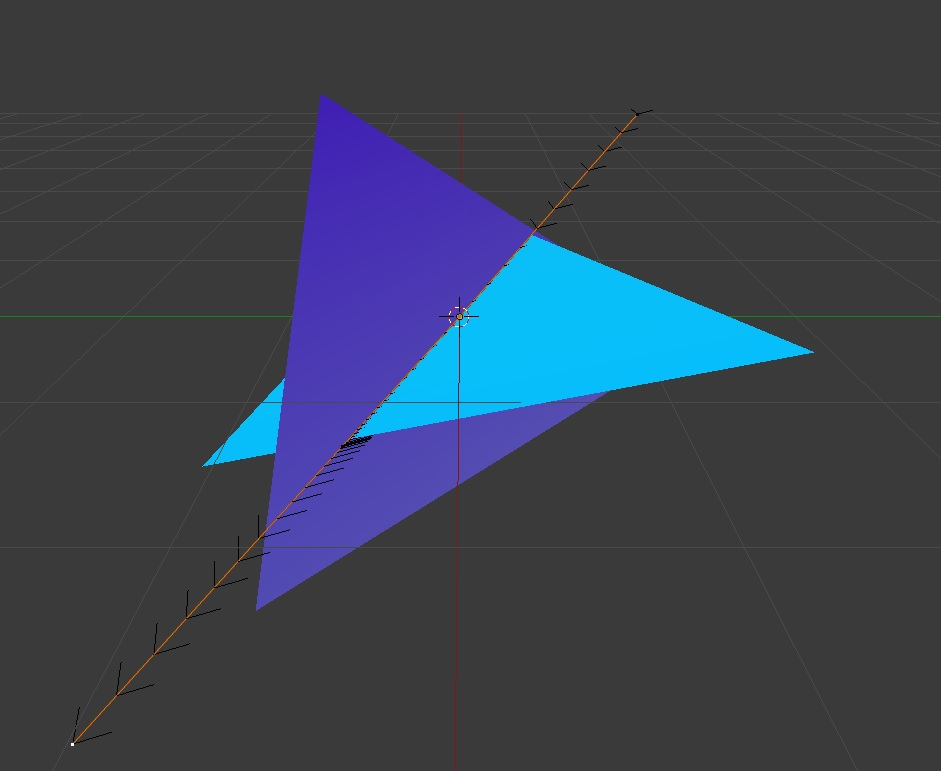
\includegraphics[width=420pt]{imgs/AsseMozzi.jpg}
	\caption{Calcolo dell'asse dei mozzi attraverso intersezione dei piani omologhi}
	\label{rot:gb:imgMozzi}
\end{figure} 

Si possono notare due triangoli i cui vertici sono i punti omologhi considerati che rappresentano i sopra detti piani omologhi. Dalla loro intersezione si definisce un asse (in arancione) passante per l'origine. Quest'ultimo è proprio l'asse dei mozzi cercato, cioè l'insieme dei punti, appartenenti ad entrambi i piani, che nella rotazione che porta alla sovrapposizione dei piani stessi rimane invariato.
% rotazione su asse dei mozzi
Individuato l'asse dei mozzi, si può effettuare una prima rotazione, intorno a tale asse, che "stende" il primo piano sul secondo. Siano $\hat{j_1}, \hat{j_1}^{'} \in \mathbb{R}^2$ i versori della proiezione di una qualsiasi coppia omologa sul piano passante per l'origine e ortogonale all'asse dei mozzi. Si può calcolare l'angolo compreso tra i due versori:
\begin{equation}
	\theta_1 = arcos(\frac{\hat{j_1} \cdot \hat{j_1}^{'}}{\| \hat{j_1}\| \|\hat{j_1}^{'}\|})
\end{equation}
Si può definire la prima rotazione, utilizzando la rappresentazione asse-angolo come:
\begin{equation}
	R_1 = Rot(asse_{mozzi}, \theta_1)
\end{equation} 

\begin{figure}[h]
	\centering
	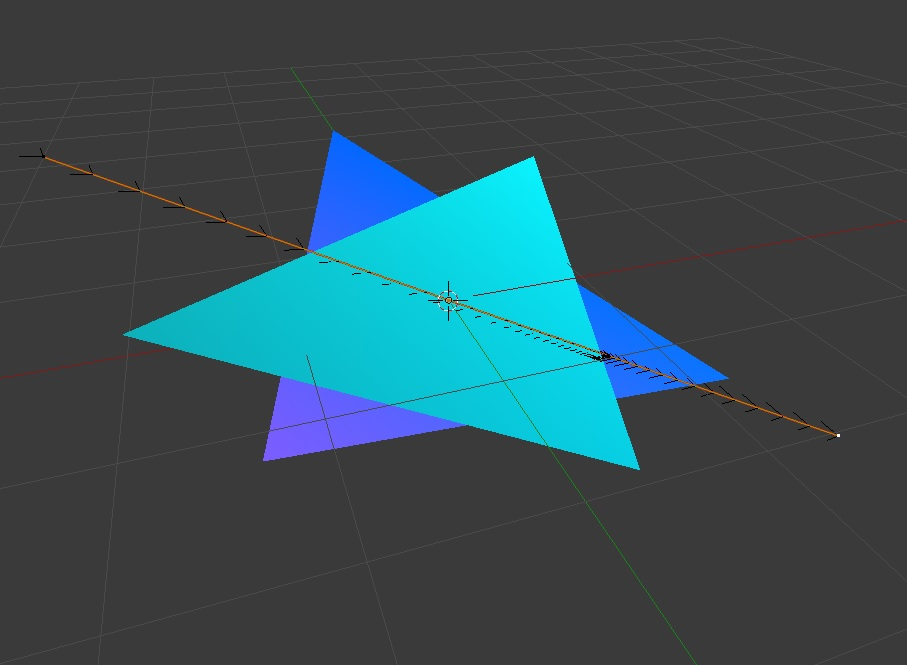
\includegraphics[width=420pt]{imgs/PianiSuStessoPiano.jpg}
	\caption{Dopo la rotazione sull'asse dei mozzi i due piani sono equi orientati}
	\label{rot:gb:samePlane}
\end{figure}

% rotazione 2d nel piano dei punti
Al netto della prima rotazione $R_1$ si è nella situazione rappresentata in figura \ref{rot:gb:samePlane}. In generale però, come è possibile evincere dalla stessa figura, i punti omologhi ancora non coincidono. Si deve individuare un ulteriore rotazione.
Si ha che i punti giacciono tutti sullo stesso piano, hanno centroide coincidente ma sono ruotati. Si può utilizzare quanto fatto nel paragrafo precedente, infatti quest'ultimo è a tutti gli effetti un caso planare.
Possiamo individuare alla stessa maniera allora:
\begin{center}
	$cos(\theta_2) = \phi_4(R_1p_1, p_1^{'}, R_1p_2, p_2^{'})/\phi_d(R_1p_1, p_1^{'}, R_1p_2, p_2^{'}), \,\,$\\
	$sin(\theta_2) = \phi_3(R_1p_1, p_1^{'}, R_1p_2, p_2^{'})/\phi_d(R_1p_1, p_1^{'}, R_1p_2, p_2^{'}),$
\end{center} 
dove $\phi_3(\cdot)$, $\phi_4(\cdot)$ e $\phi_d(\cdot)$ hanno lo stesso significato che nel paragrafo \ref{sec:groeb:plan}. Infine si calcola l'angolo
\begin{equation}
	\theta_2 = atan_2(cos(\theta_2), sin(\theta_2))
\end{equation} 
Si può definire la seconda rotazione, utilizzando la rappresentazione asse-angolo, come la rotazione intorno ad un asse unitario passante per l'origine e ortogonale ai piani.
\begin{equation}
R_2 = Rot(asse_{\bot Piano}, \theta_2)
\end{equation} 
% rotazione totale come motliplicazione delle due matrici di rotazione risultanti.
Infine possiamo individuare la matrice di rotazione risultante semplicemente pre-moltiplicando $R_1$ per $R_2$, perché trasformazioni applicate in sequenza nel riferimento mobile solidale al primo piano.
\begin{equation}
	R = R_2R_1, R \in \mathbb{R}^{3 \times 3}
\end{equation}

Trovata la matrice di rotazione, si può procedere ad individuare il vettore di traslazione relativo tra i due set. Tale vettore può essere calcolato confrontando i centroidi al netto della rotazione:
\begin{equation}
t = w_c^{'} - Rw_c, t \in \mathbb{R}^d
\end{equation}

\section{Il metodo di Kabsch}
\label{sec:kabsch}

Nel precedente paragrafo si è riusciti ad individuare una soluzione in forma chiusa per il problema in esame; tale soluzione faceva uso di un numero molto ridotto di punti omologhi per il calcolo ma un possibile errore o rumore sui set faceva si che le prestazioni della stima degenerassero.

Si presenta ora una soluzione in grado di individuare la trasformazione ottima tra i due set di punti, più robusta al rumore.

Questo metodo è stato presentato per la prima volta in \cite{bib1} ad opera di W. Kabsch, in una prima formulazione si faceva uso del concetto di moltiplicatori di Lagrange, i quali avevano un impatto prestazionale abbastanza elevato. In questa recente formulazione invece si utilizza la decomposizione SVD, strumento il cui calcolo negli ultimi anni è diventato molto efficiente.

La trasformazione che vogliamo individuare è composta, ovviamente, da una rotazione e una traslazione. Conviene iniziare con l'individuazione della prima, ragionando in modo analogo al precedente paragrafo, si comincia con il calcolo dei centroidi. Per comodità si riporta la formula per il calcolo del centroide di un set di punti:
\begin{equation}
	\label{rot:eq:cent}
	a_c = \frac{1}{N}\sum_{i = 1}^{N}a_i
\end{equation}
Si procede poi traslando i set di punti facendo si che i centroidi coincidano con l'origine:
\begin{equation}
\label{rot:eq:redef}
a_i^{'} = a_i - a_c, \, \, 
b_i^{'} = b_i - b_c
\end{equation}

Il problema ora può essere formulato come un problema di controllo ottimo: \textit{trovare la matrice ortonormale $R$ tale che la distanza di Procrustes tra i due set sia minima.} Grazie al fatto che i centroidi dei due set coincidono, tale distanza, ridefinendo come $x_i = a_i^{'}, y_i = b_i^{'}, x_i, y_i \in \mathbb{R}^d$ per comodità, può essere calcolata semplicemente come:
\begin{equation}
	\label{rot:eq:dist}
	d(x, y) =  \frac{1}{N}\sum_{i = 1}^{N} \| R x_i - y_i \|^2
\end{equation}
Si fissa quindi l'indice di costo $J = d(x, y)$. 
Si fa notare che imporre la sola ortonormalità della matrice $R$ non assicura che essa sia una matrice di rotazione propria. Infatti si dovrà fare in modo che il suo determinante sia pari a 1. In caso contrario (pari a -1) essa rappresenterebbe una rotazione impropria, cioè una componente dei punti risulterebbe "specchiata". 
Si possono rappresentare i set di punti attraverso le matrici:
\begin{equation}
	X = [x_1 \, x_2 \, ... \, x_N], Y = [y_1 \, y_2 \, ... \, y_N], X, Y \in \mathbb{R}^{d \times N},
\end{equation}
e sia $X^{'} = RX, \, \, X^{'} = [x_1^{'} \, x_2^{'} \, ... \, x_N^{'}]$ la matrice dei punti ruotati.

Possiamo allora scrivere che:
\begin{equation}
	N J = \sum_{i = 1}^{N} \| x_i^{'} - y_i \|^2 = Tr[(X^{'} - Y)^{T}(X^{'} - Y)]
\end{equation}
dove si indica con $Tr(A)$ l'operatore traccia della matrice $A$.
Grazie alla linearità dell'operatore traccia vale che:
\begin{equation}
Tr[(X^{'} - Y)^{T}(X^{'} - Y)] = Tr(X^{'T}X^{'}) + Tr(Y^{T}Y) - 2Tr(Y^{T}X^{'})
\end{equation}
Inoltre vale l'identità:
\begin{equation}
\label{rot:eq:mod}
Tr(X^{'T}X^{'}) + Tr(Y^{T}Y) = \frac{1}{N}\sum_{i = 1}^{N} \| x_i^{'} \| ^ 2 + \| y_i \| ^ 2
\end{equation}
In seguito alla (\ref{rot:eq:redef}) i punti di entrambi i set sono dei vettori centrati nell'origine. La rotazione di un vettore non può in nessun modo alterarne il suo modulo. Si può affermare allora che la quantità (\ref{rot:eq:mod}) è costante e può essere non considerata nella minimizzazione dell'indice. Pertanto, per minimizzare il suddetto indice, basterà massimizzare la quantità $Tr(Y^{T}X^{'}) = Tr(Y^{T}RX) = Tr((XY^{T})R)$.
Si fa notare che la matrice $ C = XY^{T}, \, C \in \mathbb{R}^{d \times d}$ è la matrice di cross correlazione tra i due set.

Si usa ora la decomposizione SVD della matrice $C = VSW^T$, si ha che $V, S, W^T \in \mathbb{R}^{d \times d}$ poiché $C$ è quadrata. La matrice $S$ è diagonale e i suoi elementi sono i valori singolari della matrice $C$ in ordine decrescente.
Dato che per l'operatore traccia vale che $Tr(AB) = Tr(BA)$, indicando con $A = V$ e $B = SW^TR$ è possibile scrivere:
\begin{equation}
	Tr(Y^{T}X^{'}) = Tr(VSW^TR) = Tr(SW^TRV) = \sum_{i = 1}^{d} s_iw_i^TRv_i
\end{equation}
La matrice $T = W^TRV$ è il prodotto di matrici ortonormali, sarà anch'essa ortonormale, questo vuol dire che i suoi elementi non potranno avere modulo maggiore di 1. Pertanto indicando con $T_{ii} = w_i^TRv_i$ gli elementi sulla diagonale di $T$, vale che
\begin{equation}
	Tr(Y^{T}X^{'}) = \sum_{i = 1}^{d} s_iT_{ii} \leq \sum_{i = 1}^{d} s_i
\end{equation}
 pertanto al massimo il valore della quantità $Tr(Y^{T}X^{'})$ è pari alla somma dei valori singolari $s_i$. Si deve fare in modo quindi che la matrice $T$ sia una matrice identità.
 Grazie alla proprietà di $V$ e $W^T$ di essere ortonormali, $VV^T = I, W^TW = I$, basterà scegliere:
 \begin{equation}
 	R = WV^T
 \end{equation}
Resta da risolvere un problema, cioè che in generale $det(R) = \pm 1$, il caso negativo va evitato.
Per fare ciò possiamo aggiungere il vincolo che $det(R) = 1$ al problema, ripercorrendo quanto fatto e notando che $s_1 \ge s_2 \ge \, ... \, \ge s_d$ e che
\begin{equation}
Tr(Y^{T}X^{'}) = \sum_{i = 1}^{d} s_iT_{ii} 
\end{equation}
possiamo individuare il massimo per questa quantità, rispettando il vincolo, con la scelta $T_{11} = T_{22} = \, ... \, = T_{d-1d-1} = 1, T_{dd} = -1$. Infatti, data la richiesta di ortonormalità deve valere che i $T_{ii}$ devono essere in modulo pari a 1, quindi quest'ultima è la scelta migliore possibile dato che si sottrae il valore singolare più piccolo. Basterà dunque in caso di determinante negativo, cambiare di segno all'ultimo vettore singolare destro di $W$ (l'ultima colonna della matrice $W$). Possiamo generalizzare i due casi cosi facendo:
\begin{equation}
	d = sign(det(WV^T)),
\end{equation}
\begin{equation}
	R = W
	\begin{bmatrix}
	1 \,\, 0 \,\, \cdots \,\, 0\\
	0 \,\, 1 \,\, \cdots \,\, 0\\
	\vdots\\
	0 \,\, \cdots \,\, 1 \,\, 0\\
	0 \,\, \cdots \,\, 0 \,\, d\\
	\end{bmatrix}V^T
\end{equation}

Trovata la matrice di rotazione ottima, relativa ai due set, si può procedere ad individuare il vettore di traslazione relativo tra i due set. Si procede in maniera del tutto analoga a quanto fatto nel paragrafo \ref{sec:groeb:spaz} con l'unica differenza che in questo caso, avendo effettuato una rotazione che al contrario del suddetto caso fa coincidere il secondo set sul primo, la matrice $R$ va a pre-moltiplicare il vettore $a_c$ piuttosto che $b_c$.
\begin{equation}
	t = b_c - Ra_c, t \in \mathbb{R}^d
\end{equation}
dove $b_c$ e $a_c$ sono i centroidi precedentemente calcolati.
\subsection{Robustezza ai disturbi}
\label{sec:kabsch:rumore}
La soluzione appena ottenuta, come preannunciato, oltre che ottima, risulta resistente a disturbi sulla misura. Infatti, si supponga il disturbo "bianco", cioè con valore atteso pari a 0 e il disturbo delle singole componenti indipendente dalle altre.

In prima istanza si può notare che il calcolo dei centroidi risulta corretto a patto di utilizzare un numero "abbastanza" grande di misure. Infatti, considerando $\tilde{x_i}$ la i-esima misura disturbata, si ha che
\begin{equation}
	x_c = \frac{1}{N}\sum_{i = 1}^{N} \tilde{x_i} = \frac{1}{N}\sum_{i = 1}^{N} x_i + e_i \longrightarrow \hat{x} + E[e] = \hat{x}
\end{equation}
dove con $E[e]$ si indica il valore atteso del disturbo. La precedente relazione risulta valida grazie all'ipotesi di rumore bianco, in particolare con valore atteso nullo, e l'applicazione della legge dei grandi numeri. Aumentando il numero dei campioni cresce la probabilità di convergenza della media campionaria verso il valore atteso.

Il calcolo della matrice di cross-correlazione avviene sempre a mezzo di tali misure, se consideriamo una qualsiasi componente della matrice $C$ si ha che:
\begin{equation}
	c_{ij} = \sum_{k = 1}^{N}  \tilde{X_{ik}} \tilde{Y_{kj}} \longrightarrow \sum_{k = 1}^{N} X_{ik} Y_{kj} + (\cdots) \begin{bmatrix}
	E[e_x] \\
	E[e_y]
	\end{bmatrix} = \hat{c_{ij}}
\end{equation}
dove la quantità tra parentesi è una combinazione delle misure.

A patto di usare un buon numero dei campioni si ha quindi un aumento della probabilità di individuare i centroidi e la matrice di cross-correlazione "veri". Il calcolo precedente, produce allora un risultato "vero", cioè relativo ai centroidi e la matrice di cross-correlazione privi di rumore.

In caso di rumore, l'errore quadratico prodotto dal calcolo può essere un indice del rumore presente sulle misure.

Al tendere del numero di campioni all'infinito, anche in caso di rumore, l'algoritmo individuato produce un risultato corretto con probabilità 1.



%matrice di covarianza stimata converge a quella verà perchè su ogni elemento ci va la somma fino a N del disturbo in più che converge a 0
\chapter{Visione artificiale}
\label{chap:visione}

\begin{minipage}{12cm}\textit{In questo capitolo verrà trattato il problema della generazione dei set di coppie di punti omologhi usando tecniche di visione. In particolare si utilizzeranno tecniche di Feature Detection e stereoscopia.}
\end{minipage}

\vspace*{1cm}

Nel capitolo \ref{chap:visualObs} si è accennato agli strumenti che sarebbero stati usati al fine della generazione dei suddetti set. In questo capitolo si procederà ad illustrarne il funzionamento con maggior dettaglio e si fornirà una possibile soluzione al problema. Conviene definire per primo il problema che si vuole affrontare.

\begin{prob}
	\label{prob:vis:gensets}
	Sia un osservatore mobile dotato di almeno due fotocamere. Si supponga ancora capace di "catturare", attraverso le suddette fotocamere, coppie di foto in diversi istanti (anche regolari). Allora: 
	\begin{enumerate}
		\item è possibile, utilizzando le informazioni fornite dalle fotocamere, calcolare le coordinate spaziali (in $\mathbb{R}^3$) di un punto del mondo (o più di uno) nel sistema di riferimento solidale all'osservatore?
		\item dato un punto del mondo (o più di uno) per il quale si è riusciti a calcolarne le coordinate spaziali, è possibile individuare lo stesso punto, in un altro istante del tempo, se l'osservatore si è mosso e se lo stesso è ancora visibile?  
	\end{enumerate}
\end{prob}

\section{Feature Detection e Matching}
\label{sec:feature}
Per \textbf{Feature Detection} o \textbf{individuazione dei punti chiave} in italiano, si intende un particolare settore facente parte della branca della visione artificiale, il cui scopo è quello di per l'appunto l'individuazione, la descrizione e il confronto delle Feature. Ma che cosa è una Feature?
In generale risulta difficile fornire una definizione chiara di cosa è una \textbf{Feature} o \textbf{Punto chiave}, può dipendere ad esempio dall'algoritmo che si utilizza o da scelte implementative.


\begin{figure}[h]
	\centering
	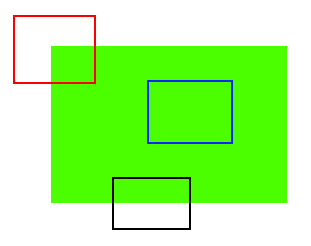
\includegraphics[width=420pt]{imgs/feature_simple.png}
	\caption{Individuazione delle Features.}
	\label{vis:feature:detect}
\end{figure} 

Si faccia ad esempio riferimento alla figura \ref{vis:feature:detect}, si supponga di dover individuare una buon punto chiave, il quale possa essere facilmente riconosciuto e riposizionato. Si consideri per prima la porzione di immagine evidenziata dal riquadro blu; è chiaro che qualora si dovesse scegliere dove posizionare tale blocco, si avrebbero un numero elevatissimo di possibilità ed in nessun caso si potrebbe avere al certezza di un buon posizionamento. Si consideri allora il blocco nero, in questo caso il numero delle possibilità è sicuramente inferiore, infatti esso può essere posizionato solo nel lato inferiore del rettangolo verde in figura. Infine si consideri il blocco rosso, è chiaro che quello in figura è l'unico punto in cui esso può essere posizionato.
L'esempio precedente fornisce un importantissimo spunto ri riflessione su cosa può essere una Feature e cosa no. Infatti sicuramente una porzione di immagine uniforme non può essere un punto chiave; se invece si considerano dei contorni di un oggetto la situazione migliora. In particolare se si considera il contorno di un oggetto e se ne sceglie un punto che abbia una forma o pattern particolare, come ad esempio uno spigolo di un oggetto, risulta molto più facile un eventuale riconoscimento. 

Ovviamente l'esempio precedente risulta estremizzato. Infatti, in un caso reale, le Feature possono essere ruotate e/o scalate e questo complica il problema. Al contempo però, il mondo reale risulta più dettagliato e risulta più difficile avere uno stesso pattern in punti diversi.

Si è fornita, quanto meno in modo informale, una definizione di Feature. Nei prossimi paragrafi con ordine si illustreranno tre algoritmi: il primo adibito all'individuazione delle features, il secondo viene impiegato per la generazione dei descrittori (che come si vedrà sono utilizzati per distinguere i punti chiave in base alle informazioni fornite dall'immagine) ed il terzo è sostanzialmente un matcher. 

%\subsection{Definizioni e problema}
%\label{sec:det:def}


\subsection{L'algoritmo FAST}
\label{sec:det:fast}

\subsection{L'algoritmo BRIEF}
\label{sec:det:brief}

\subsection{Brute Force matching}
\label{sec:det:bmmatch}


\section{Stereoscopia}
\label{sec:stereo}


%\subsection{Definizioni e problema}
%\label{sec:stereo:def}


\subsection{Modello matematico del sensore fotografico}
\label{sec:stereo:modello}


\subsection{Ricostruzione 3D}
\label{sec:stereo:ric3d}


\section{Soluzione al problema}
\label{sec:vision:solution}



\chapter{Implementazione Framework}
\label{chap:impl}

\begin{minipage}{12cm}\textit{In questo capitolo si illustreranno gli aspetti tecnici del problema in esame: la scelta delle librerie, i problemi riscontrati e le soluzioni intraprese. In particolare si porrà particolare accento sull'efficienza al fine di rendere lo stimatore applicabile in contesti real-time.}
\end{minipage}

\vspace*{1cm}

\section{Strumenti utilizzati}
\label{sec:tools}


\subsection{OpenCV}
\label{sec:tools:opencv}

\subsection{CUDA}
\label{sec:tools:cuda}



\section{Lo sviluppo}
\label{sec:sviluppo}

\subsection{Ambiente di sviluppo e target}
\label{sec:dev:ambiente}

\subsection{Obbiettivi di sviluppo e soluzioni}
\label{sec:dev:obj}



\chapter{Test}
\label{chap:test}

\begin{minipage}{12cm}\textit{blabla..}
\end{minipage}

\vspace*{1cm}

\section{Il motore grafico Unity3D}
\label{sec:unity}


\section{Vantaggi e svantaggi di una validazione con motore grafico}
\label{sec:valid}

\section{Risultati ottenuti}
\label{sec:perf}



\chapter{Conclusioni e sviluppi futuri}

In questo lavoro di tesi, si sono toccati diversi ambiti: dalla geometria alla stima, dalla visione stereoscopica fino al riconoscimento delle feature. Si è inoltre effettuato un grosso lavoro di progettazione e implementazione, si sono dovuti prima di tutto individuare i problemi da affrontare per poi, ovviamente, fornirne una soluzione. L'obiettivo iniziale era del tutto differente ed il risultato ottenuto è stato un susseguirsi di idee e tentativi. Talvolta il risultato poteva sembrare troppo lontano, ma procedendo a testa bassa, dividendo il problema in diversi più piccoli, da affrontare uno alla volta, si è riuscito a fornire una soluzione ad ognuno di essi. Si è potuto studiare strumenti innovativi, sperimentarli e talvolta scartarli per arrivare alla fine ad un prodotto finito, funzionante. Sicuramente il lavoro svolto ha ancora grossi margini di miglioramento, si dovrà lavorare sulla stabilità del software, sperimentarlo nel mondo reale e nuove funzionalità o algoritmi potranno essere inseriti. Grazie all'architettura progettata tale aspetto risulterà più semplice, si potranno modificare singole parti del software, fornire implementazioni diverse. Eventualmente, più persone potranno collaborare, migliorare il prodotto insieme e condividere quanto fatto. 

In conclusione, si sono toccate differenti materie al fine di convergere verso un prodotto funzionante, aperto e aggiornabile.

Si è fornito un possibile approccio risolutivo basato sull'utilizzo di strumenti appartenenti a campi differenti: stima, geometria e visione artificiale. Si sono forniti gli strumenti atti a rendere il lavoro svolto comprensibile anche da un lettore non ferrato in questi campi, nella speranza che esso possa essere di ispirazione e possa servire da punto di partenza per sviluppi futuri. 

Il problema è stato diviso in uno di stima e uno di visione. Nel capitolo \ref{chap:stima} si è appunto studiato il primo problema, si sono presentate due differenti soluzioni: la prima basata sull'utilizzo di tecniche algebriche e geometriche. Si è pertanto studiato argomenti non facenti parte del corso di studio, quali le basi di Groebner e la teoria dell'eliminazione. Si è utilizzato il software Macaulay per applicare tali concetti e si è ottenuta una soluzione capace di stimare la matrice di rotazione e il vettore di traslazione nel caso planare. Tale soluzione è stata poi estesa al caso spaziale utilizzando concetti di geometria. In particolare si è dimostrato, in maniera differente e in accordo al risultato di Denavit ed Hartemberg, che un qualsiasi spostamento può essere raggiunto con soli due traslazioni e due rotazioni. Si è poi adattato un algoritmo, detto di Kabsch, utilizzato spesso in ambienti bio-informatici, al fine di ottenere una soluzione, in forma chiusa, più robusta ai disturbi di misura. Se ne è data la prova e nel capitolo \ref{chap:implTest} si mostrato il funzionamento numerico.

Il secondo grande problema, presentato nel capitolo \ref{chap:visione}, ha riguardato la generazione di "riferimenti" da poter utilizzare nella stima. Il problema è stato affrontato utilizzando e studiando tecniche innovative appartenenti al campo della visione artificiale. Infine si è fornita una procedura costruttiva.

Negli ultimi due capitoli si è proceduto a descrivere gli aspetti implementativi e di test delle prestazioni. Si è ottenuto un architettura snella, veloce e modulare. Si sono fornite poi diverse implementazioni, facenti uso di caratteristiche hardware diverse, per gli algoritmi presentati.

In futuro, si prevede di continuare lo sviluppo e di trovare risposte ad ulteriori problemi riscontrati sia in sede teorica che in fase di test. Ad esempio si potrebbe:
\begin{itemize}
	\item Prevedere la possibilità di gestire diversi oggetti dinamici nella scena. Questo potrebbe essere fatto in differenti maniere:
	\begin{itemize}
		\item agendo a livello della stima ed individuando ulteriori algoritmi in grado di risolvere un problema che si potrebbe chiamare multy body Procustes. In cui si deve trovare la disposizione ottima di un gruppo di oggetti posti a confronto.
		\item agendo a livello di identificazione dei punti, escludendo i punti chiave appartenenti ad oggetti ritenuti mobili. Si potrebbe fare tale distinzione utilizzando tecniche di machine learning e riconoscimento degli oggetti.
	\end{itemize}
	\item Costruire un prototipo e sperimentarne il funzionamento in un contesto reale.
	\item Migliorare l'integrazione con Unity che allo stato attuale, per motivi tecnici e prestazionali, è stato utilizzato al solo fine di generare un input visivo offline. Con una migliore integrazione, si potrebbe fare in modo che un eventuale agente possa "navigare" e compiere scelte di controllo all'interno del mondo virtuale.
	\item Migliorare quanto fatto, rendendo il software sempre più veloce e meno affetto da errori.
\end{itemize}








% ELENCO DELLE FIGURE (OPZIONALE)
\addcontentsline{toc}{chapter}{Elenco delle figure}
\listoffigures

% BIBLIOGRAFIA
\addcontentsline{toc}{chapter}{Bibliografia}
\begin{thebibliography}{9}
        \bibitem{bib1}W. Kabsch,
            \emph{``A Solution for the Best Rotation to Relate Two Sets of Vectors, 32, 922-923''},
          Acta Crystallographica, 1976.
        
        \bibitem{bib2}E. Rosten, T. Drummond,
        \emph{``Machine learning for high speed corner detection, vol. 1, 430–443''},
        9th European Conference on Computer Vision, 2006.
       
       	\bibitem{bib3}E. Rosten, R. Porter, T. Drummond,
       	\emph{``Faster and better: a machine learning approach to corner detection, vol. 32, 105-119''},
       	IEEE Trans. Pattern Analysis and Machine Intelligence, 2010.
       	
       	\bibitem{bib4}M. Calonder, V. Lepetit, C. Strecha, P. Fua,
       	\emph{``BRIEF: Binary Robust Independent Elementary Features, vol. 6314, 778-792''},
       	11th European Conference on Computer Vision (ECCV), Heraklion, Crete. LNCS Springer, 2010.
       	
      
       	
\end{thebibliography}
\end{document}
